\documentclass[xcolor=dvipsnames, 13pt]{beamer}
\usepackage{amsmath, amsfonts, epsfig, xspace, relsize}
\usepackage{algorithm,algorithmic, graphicx}
\usepackage{pstricks,pst-node}

%\usecolortheme[named=NavyBlue]{structure}
\usepackage{equation}
%\usepackage{mathtools}
\usepackage{relsize}
\usepackage{IEEEtrantools}
\newcommand{\non}{\nonumber}
\usepackage{fancyhdr}
\usepackage{fancyvrb}
\usepackage{booktabs}
\usepackage{psfrag}
\usepackage{amsbsy,amsgen,amssymb,equation}
\usecolortheme[rgb={0.6, 0.1, 0}]{structure}
\usetheme{Madrid}
 \usepackage{graphicx}
  \DeclareGraphicsExtensions{.pdf,.png,.jpg,.jpeg,.mps}
%\usepackage{beamerthemeshadow}
\usepackage{fontspec}  %加這個就可以設定字體 
%\setsansfont{Georgia}
\usepackage{xecjk} 
 
\XeTeXlinebreaklocale "zh" 
\XeTeXlinebreakskip = 0pt plus 1pt 
%\usetheme{CambridgeUS}  % 另外一種 樣版
%\setCJKmainfont[BoldFont=Adobe Heiti Std,ItalicFont=Adobe Kaiti Std]{Adobe Song Std}
%\setCJKmainfont{YouYuan}
\setCJKmainfont[BoldFont=Adobe Heiti Std,ItalicFont=Adobe Kaiti Std]{YouYuan}
\setCJKfamilyfont{lishu}{LiSu}
\setCJKfamilyfont{kaiti}{Adobe Kaiti Std}
\setCJKfamilyfont{zhfs}{Adobe Fangsong Std}
\newcommand*{\lishu}{\CJKfamily{lishu}}
\newcommand*{\kaiti}{\CJKfamily{kaiti}}   % 楷体
\newcommand*{\fangsong}{\CJKfamily{zhfs}} % 仿宋
\setsansfont{Garamond}
\title[信度與效度]{\kaiti{變數之信效度意義以及檢測}}
%\date{}


\author [CHT] {\fangsong 蔡佳泓\\
\bigskip
國立政治大學選舉研究中心\\
\bigskip
\texttt{tsaich@nccu.edu.tw}
}
\institute {NCCU}

\date[]{2015 年 3 月 12 日} 

\begin{document}
\maketitle
\begin{frame}\frametitle{大綱}
\normalsize
%\begin{enumerate}
\tableofcontents
%\end{enumerate}
\end{frame}

\section{研究的基本概念}

\begin{frame}{研究的基本概念}

\begin{itemize}
\item<1-> 分析單位
\item<2-> 變項
\item<3->  相關
\item<4-> 因果關係
\end{itemize}
\end{frame}

\begin{frame}\frametitle{分析單位}
\begin{itemize}
\item 個人:所有成人、65 歲以上成人、孕婦等等
\item 群體:學校的班級、醫院的單位
\item 個人有可能受到群體的影響;個人的差異有可能同時來自群體以及個人本身
\item 有分析單位才能確定測量的方式。例如:個人的身高、體重、生活品質必須以個人為單位進行測量。
一個國家的醫療品質、生育率、離婚率等等則是以國家為單位測量。
\end{itemize}
\end{frame}

\begin{frame}\frametitle{變數}
\begin{itemize}
\item 抽象概念例如「生活品質」、「顧客滿意度」需要轉換成可測量的概念,測量之後得到變數。
\item 例如:「顧客滿意度」就是對於品質以及付出價格相比在心理上的滿意程度。
\item 一個概念如果有不止一個面向,可以考慮用一個以上的測量。
\item 例如:「心理健康」測量包括自己的生理狀況評估、與家人、朋友相處情況等等。
\item 例如:「休閒運動」測量包括去過幾次美術館、每週做幾次明顯的流汗運動等等。
\end{itemize}
\end{frame}

\begin{frame}\frametitle{相關}
\begin{itemize}
\item 定義:兩個變數有一起變動的傾向。
\item 例如:「挫折感」產生攻擊的傾向。
\item 例如:做運動可以降低焦慮感。
\item 相關的背後應該有理論。例如,科學家發現只要你的身體有在活動,看待周遭環境的看法就會改變,變得不再那麼有威脅、有攻擊性,也不會覺得有那麼多不安全感。
\end{itemize}
\end{frame}
\begin{frame}\frametitle{因果關係}
\begin{itemize}
\item 如果兩個變數有相關,而且可以確定變數 X 是造成變數 Y 變動的唯一變數,X 與 Y 有因果關係。
\item 例如:隨機分派兩組成年人。實驗組除了喝水之外,每天喝兩杯咖啡,控制組每天只喝水。兩組的唯一差異來自
於喝咖啡,因此咖啡跟心跳或是血壓之間可能有因果關係。
\end{itemize}
\end{frame}

\begin{frame}{因果關係}
\begin{itemize}
\item 以方程式表示因果關係如下:
\begin{IEEEeqnarray}{rcl}
 Y & = & \beta_{0}+\beta_{1}X_{1}+\beta_{2}D
\label{eq:multreg2} 
\end{IEEEeqnarray} 
其中 \\
\begin{equation}
D=\begin{cases}
1 & \text{喝兩杯咖啡}\\
0 & \text{其他}
\end{cases}
\end{equation}
\hspace{15pt}當 $D=1$,式 \ref{eq:multreg2} 可改寫為:
\begin{IEEEeqnarray}{rcl}
Y & = & \beta_{0}+\beta_{1}X_{1}+\beta_{2} \non\\
 & = & (\beta_{0}+\beta_{2})+\beta_{1}X_{1} 
\label{eq:multregd1} 
\end{IEEEeqnarray} 
\hspace{15pt}當 $D=0$,式 \ref{eq:multreg2} 可改寫為:
\begin{IEEEeqnarray}{rcl}
Y & = & \beta_{0}+\beta_{1}X_{1}+\beta_{2}\cdot 0 \non\\
 & = & \beta_{0}+\beta_{1}X_{1} 
\label{eq:multregd2} 
\end{IEEEeqnarray} 
\item 式 \ref{eq:multregd2} 以及式 \ref{eq:multregd1} 相減等於 $\beta_{2}$,也就是類別變數 $D$ 的作用。
\end{itemize}
\end{frame}

\section{測量的概念}
\begin{frame}\frametitle{何謂測量}
\begin{itemize}
\item 根據變項,以及一定的規則,決定研究對象所有的值。測量必須盡可能地得到與對象一致的值。
\item 可以用觀察或是自我報告進行測量。
\item 例如:用體重以及身高,測量身體質量 (BMI)
\item 例如:用自我檢查表測驗視力。
\item 例如:以一個假設世代的育齡婦女,按照目前生育的年齡水準,一生所生育的嬰兒數,測量總生育數。
\end{itemize}
\end{frame}

\begin{frame}\frametitle{測量的層次}
\begin{itemize}
\item 名目:如果測量的目的是分類,屬於名目層次的測量
\item 順序:如果測量的目的是排名次,屬於順序層次的測量,例如高、中、低。過去血壓超過140/90mmHg(毫米汞柱),才是高血壓,現在標準則降低為 120/80mmHg
\item 等距:分數之間的距離相等,但是沒有絕對零點,例如智力沒有 0,所以不能說某人智力是另一人的倍數。
\item 比值:除了等距之外還有絕對零點,例如講話的長度。
\end{itemize}
\end{frame}

\section{信度}
\begin{frame}{何謂信度?}
\begin{enumerate}
\item 測量的工具應該盡可能地測量到態度或是行為的真實分數,但是真實分數觀察不到,而是由測量分數與誤差所構成:
\begin{block}{信度公式}
X = T + E \\
X:觀察分數 \\
T:真實分數 \\
E:誤差
\end{block}
\item 當誤差為 0,測量工具完美地測量到真實的分數。但是施測時的環境或者是受訪者當時的狀況不一樣,
有可能產生測量的誤差。
\end{enumerate}
\end{frame}
\begin{frame}{影響信度的因素}
\begin{itemize}
\item 受訪者的變異程度;變異程度越高,信度越高。
\item 信度理論上可以表示總變異量減去誤差分數的變異量,或者表示為:
\begin{block}{信度的公式}
\begin{equation*}
\mathlarger{r_{xx} = \frac{S_{x}^2}{S_{x}^2} - \frac{S_{e}^2}{S_{x}^2} = 1- \frac{S_{e}^2}{S_{x}^2} }
\end{equation*}
\end{block}
\item 如果 $S_{e}^2 = 0$,也就是沒有誤差,信度等於 1。
\item 因此信度的範圍是 0 到 1。
\end{itemize}
\end{frame}
\subsection{估計信度的方法}
\begin{frame}{估計信度的方法}
\begin{itemize}
\item 重測
\item 複本
\item 內部一致性
\end{itemize}
\end{frame}

\begin{frame}{重測}
\begin{itemize}
\item 對同一群人在不同時間進行同一測量,得到的相關分數稱為\textcolor{blue}{重測信度係數 (test-retest reliability
coefficient)}。
\item 兩次測量間隔的時間如果太長,有可能測量到其他的誤差,例如受訪者本身的態度、身心狀況改變,測量的信度可能低估。間隔的時間太短,受訪者有可能記憶上一次的答案,測量的信度可能高估。
\item 重測如果多次,理論上應該會得到一個平均分數,如果誤差是隨機的,平均之後誤差會消失。
\end{itemize}
\end{frame}
\begin{frame}{相關係數}
\begin{block}{Pearson 相關係數}
$r=\mathlarger {\frac{\sum_{i=1\sim n} (X_{i}-\bar{X})(Y_{i}-\bar{Y})}{\sqrt{\sum (X_{i}-\bar{X})^2} \sqrt{ \sum (Y_{i}-\bar{Y})^2} }}$
\end{block}
\begin{itemize}
\item 介於 -1 與 1 之間。
\item 0$\sim$1 表示正相關
\end{itemize}
\end{frame}
\begin{frame}[fragile]{相關係數}
%\begin{itemize}
以美國五十個州的每人平均收入與不識字率進行相關分析,其中平均收入取對數。
%\end{itemize}
\bigskip
\begin{Verbatim}[frame=single,label=\textit{R code}]
cor(state$Illiteracy, log(state$Income))
[1] -0.4804337
\end{Verbatim}
\end{frame}

\begin{frame}{散佈圖}
\begin{figure}
\begin{center}
\includegraphics[width=2.8in,height=2.9in]{scatter.png}
\end{center}
\end{figure}
\end{frame}
\begin{frame}\frametitle{複本信度}
\begin{enumerate}
\item 從一組題目之中,選取部分題目進行測量,前後兩次的測量的相關係數,可得到複本信度。
\item 因為測量內容不完全相同,但是本質相同,所以得到的相關可以反應測量的信度
\item 複本信度需要足夠的題目可供挑選。
\end{enumerate}
\end{frame}

\begin{frame}{內部一致性}
\begin{enumerate}
\item 折半方法:把測量題目隨機分為一半,然後計算各一半測驗分數的相關係數。
\begin{block}{Spearman-Brown formula}
$\mathlarger{\frac{nr}{1+(n-1)r}}$ \\
$r$:原測驗的信度 \\
$n$:測驗加長或是減短倍數 
\end{block}
\item 當 $n$ = 2,就是測驗加倍,可獲得折半的信度。
\end{enumerate}
\end{frame}

\begin{frame}\frametitle{計算折半信度範例}
假設有五名受訪者填寫問卷,其中四題的結果如下:
\begin{table}
\begin{tabular}{l | r  r  r  r  | r  r}
\hline
Name & I1 & I2 & I3 & I4 & odd & even \\
\hline
A & 1 & 1 & 1 & 1 & 2 & 2 \\
B & 1 & 0 & 1 & 1 & 2 & 1 \\
C & 1 & 0 & 1 & 0 & 2 & 0 \\
D & 0 & 0 & 1 & 0 & 1 & 0 \\
E & 0 & 0 & 0 & 0 & 0 & 0 \\
\hline
\end{tabular}
\end{table}
\end{frame}
\begin{frame}[fragile]{計算折半信度}
以相關係數計算原始信度:
\bigskip
\begin{Verbatim}[frame=single,label=\textit{R code}]
odd<-c(2,2,2,1,0); even<-c(2,1,0,0,0)
cor(odd, even)
# 0.5625
\end{Verbatim}
假設增加一倍的數目,計算 Spearman-Brown 信度
\bigskip
\begin{Verbatim}[frame=single,label=\textit{R code}]
spearman.brown(.5625, 2)
# 0.72
\end{Verbatim}
\end{frame}
\begin{frame}\frametitle{Cronbach's $\alpha$ 公式}
\begin{itemize}
\item 1951 年 Cronbach 提出 $\alpha$ 係數,國內翻譯為柯能畢曲 $\alpha$ 係數。
\begin{block}{Cronbach's $\alpha$}
\[\alpha=\frac{k}{k-1}\cdot{1-\frac{\sum \sigma^2_{i}}{\sum \sigma^2}} \]
k:題目數 \\
$\sigma^2_{i}$:每一道題目的變異數\\
$\sigm^2$:所有觀察值的分數的變異數
\end{block}
\item 也可以轉換為相關係數
\begin{block}{Cronbach's $\alpha$}
\[\alpha=\frac{k\cdot{\bar{r}}}{1+(k-1)\cdot{\bar{r}}} \]
$\bar{r}$:平均問項間相關係數
\end{block}
\item $\alpha$ 為量表的總共變異量可歸因於同一來源或因素的比例。
\end{itemize}
\end{frame}


\begin{frame}\frametitle{計算 Cronbach's $\alpha$ 範例}
假設有十名受訪者填寫問卷,其中五題的結果如下:
\begin{table}
\begin{tabular}{l | r  r  r  r  r }
\hline
Name & I1 & I2 & I3 & I4 & I5 \\
\hline
A & 0 & 0 & 0 & 0 & 0 \\
B & 0 & 0 & 0 & 0 & 0 \\
C & 0 & 0 & 0 & 0 & 1 \\
D & 0 & 0 & 0 & 1 & 1 \\
E & 0 & 0 & 1 & 1 & 1 \\
F & 0 & 1 & 1 & 1 & 1 \\
G & 1 & 1 & 1 & 1 & 1 \\
H & 1 & 0 & 1 & 1 & 1 \\
I & 0 & 0 & 0 & 1 & 1 \\
J & 0 & 1 & 1 & 1 & 1 \\
\hline
\end{tabular}
\end{table}
\end{frame}

\begin{frame}[fragile]\frametitle{計算 Cronbach's $\alpha$ }
\begin{Verbatim}[frame=single,label=\textit{R code}]
c<-apply(x, 1, function(x) sum(x)) # 計算每一列的和
y <- var(c) 					 # 計算每一列和的變異數
# y=3.16
h<-apply(x, 2, function(x) var(x)) # 計算每一行的變異數
si<-sum(h)					# 總和	
# si = 1.1
k=5						# 題數	
cronbach<-(k/(k-1))*(1-(si/y))   
# 0.8157
\end{Verbatim}
或者是用 \texttt{R} 的 CTT 套件之中的 \texttt{reliability} 指令:
\begin{Verbatim}[frame=single,label=\textit{R code}]
reliability(x)

# Coefficient Alpha 
# 0.816 
\end{Verbatim}
\end{frame}
\begin{frame}\frametitle{信度與效度}
\begin{figure}
\begin{center}
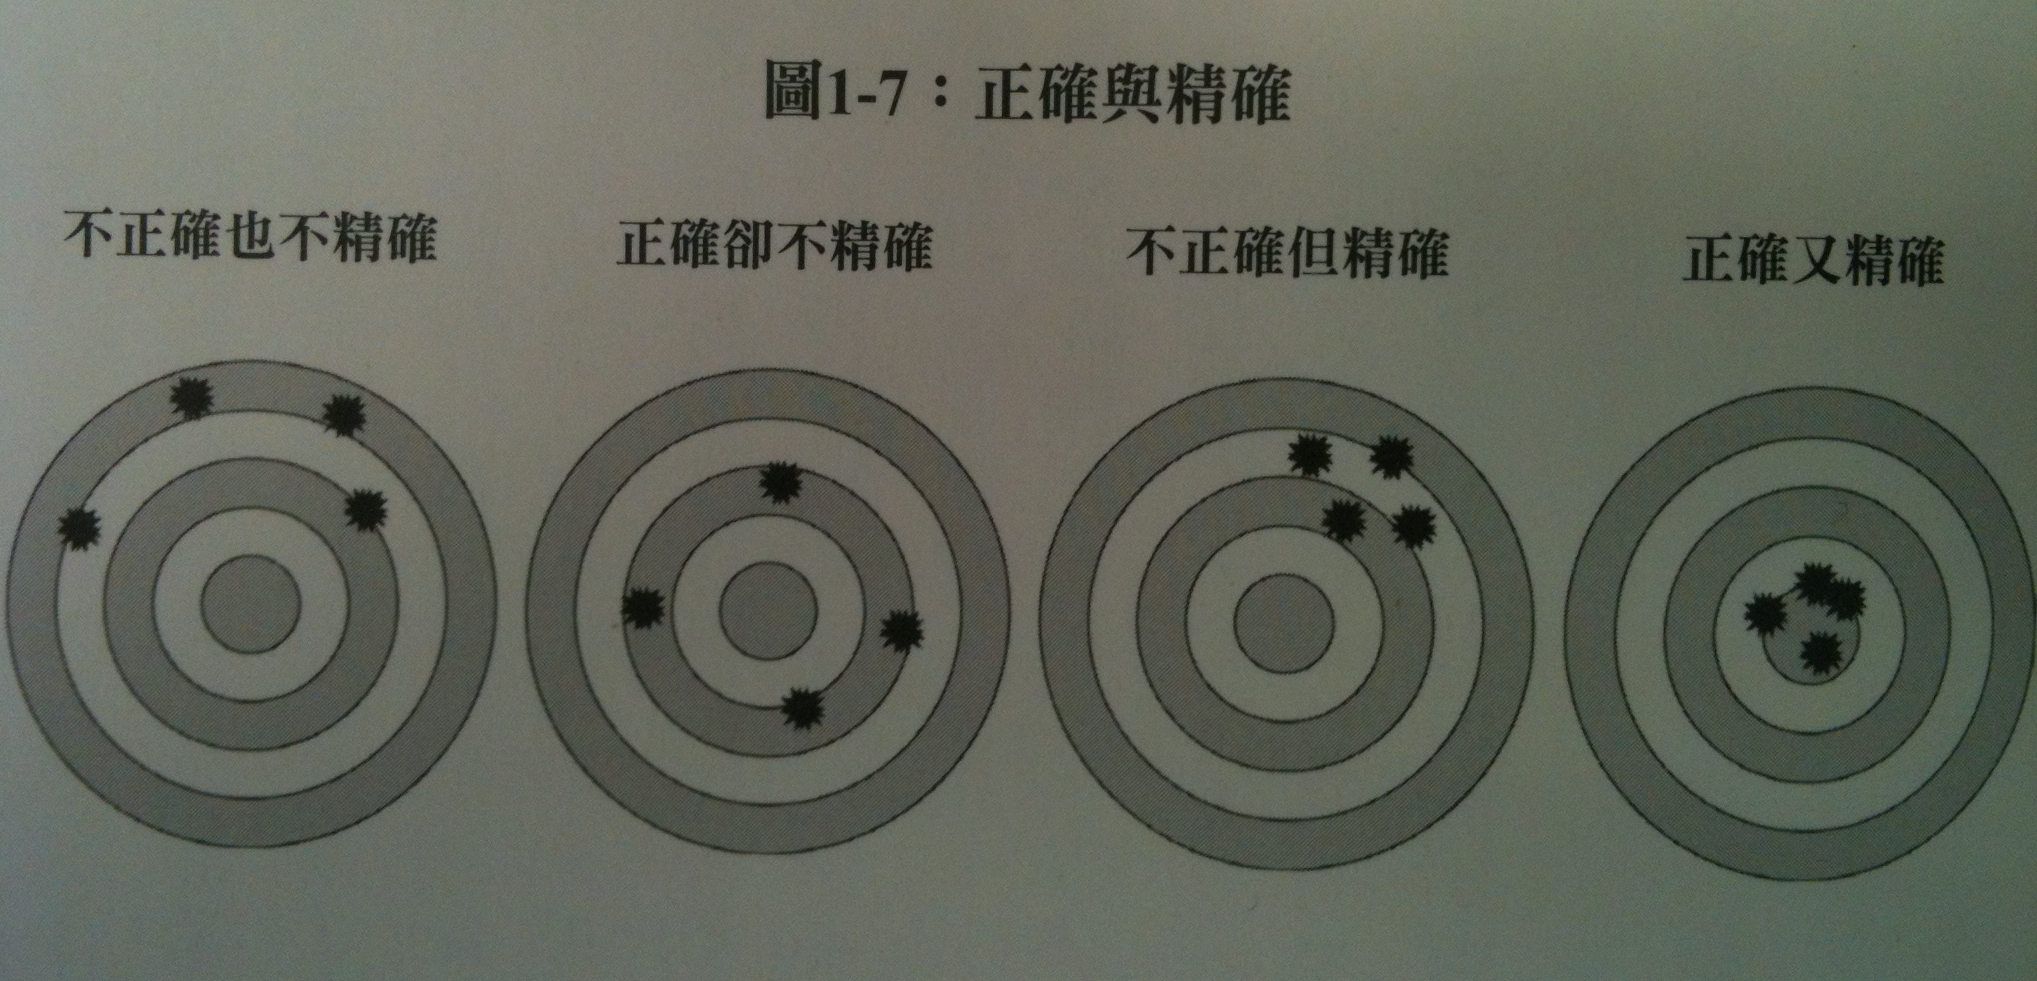
\includegraphics[width=3.2in,height=2.9in]{validityplot.png}
\end{center}
\end{figure}
\end{frame}
\section{效度}
\begin{frame}{何謂效度}
\begin{itemize}
\item 正確地測量到心目中的概念
\item 例如:智力定義為聰明的程度,因此,好的智力測驗應該能夠測量聰明的程度。智力測驗的分數越高,應該
表現出越高的推理能力。但是智力測驗可能無法測量到記憶力。
\item 效度無法直接測量,只能間接地推論。
\item 只有相對的校度,要由研究者來選擇哪一種測量比較適合。
\end{itemize}
\end{frame}

\begin{frame}{效度的類型}
\begin{enumerate}
\item 表面效度
\item 內容效度
\item 建構效度
\item 構念效度
\end{enumerate}
\end{frame}
\begin{frame}{表面效度}
\begin{itemize}
\item 從測量的字面意義判斷是否具有效度
\item 例如:健康狀況可以用如下的題目測量(社會變遷調查):
\begin{enumerate}
\item 請問您抽煙嗎?
\item 請問您抽煙抽了多少年?
\item 請問您喝酒嗎?
\item 請問您多常做至少持續20分鐘會讓您流汗或呼吸較平常急促的運動?
\item 請問您嚼不嚼檳榔?
\item 請問您的身高?(公分,請輸入整數)
\item 請問您的體重?(公分,請輸入整數)
\item 請問您認為自己是屬於何種體型?
\end{enumerate}
$\dots$
\end{itemize}
\end{frame}
\begin{frame}{內容效度}
\begin{itemize}
\item 和表面效度類似,但是進一步考慮概念的面向,判斷每一個題目是否符合測量的目標,
內容是否周延、具代表性、適切性、並確實包含所欲測量主題的內涵。
\item 為了確認內容效度,最好依據適當的文獻進行理論的探索。如果可以的話,用複本信度確認效度
\end{itemize}
\end{frame}
\begin{frame}{建構效度}
\begin{itemize}
\item 用一個外在的測量與我們建立的測量進行相關分析,相關係數越高,代表測量具有效度。又可分為同時與預測效度
\item 同時效度:在同一個時間,進行兩種測量,其中一個已經公認具有效度,或稱為效標,另一個是不確定效度的測量。如果兩者出現理論上預期的相關,那麼可以確定測量的效度。心理健康與憂鬱症量表應該有高度相關,後者已經具有公認的效度,可以用來檢測前者的效度。
\item 預測效度:在測量進行之後一段時間,分析與效標之間的相關程度。如果相關程度高,代表測量具有效度。例如,國中三年級的成績,可以評估國中二年級的學習測量。
\end{itemize}
\end{frame}
\begin{frame}\frametitle{構念效度}
\begin{itemize}
\item 用更周延的理論架構,衡量測量能夠符合理論上的結構的程度。
\item 根據理論,可以提出一些假設,而測量應該要符合理論的各種預期。
\item 智力應該:
\begin{enumerate}
\item 隨著年齡而增長
\item 可以預測學業成就
\item 應該會受到不同教學方法的影響
\end{enumerate}
\item 因此智力測量的結果應該符合以上的預期,才具有構念效度。
\item 如果沒有得到預期的發現,有可能是:
\begin{enumerate}
\item 沒有測量到所要測量的對象;
\item 理論架構有缺陷;
\item 研究設計沒有考慮其他潛在因素的影響。
\end{enumerate}

\end{itemize}
\end{frame}
\subsection{因素分析}
\begin{frame}\frametitle{因素分析}
\begin{itemize}
\item 因素分析可以縮減資料的面向 (dimensionality)。原本一筆資料可能有 A、$\dots$、Z 等等變數,透過因素分析,也許縮減成三個變數,仍然可以包含大部分資料中的變異程度。
\item 一個測量如果具有構念效度,不同變數應該會測量到相近的特質,或者是潛在的結構。
\item 例如:學生對於老師的印象,可能來自老師對學生的鼓勵、互動,也可能來自於老師的上課技巧、評分方式。因此,要測量學生對老師的印象,應該包含至少這兩個因素,而設計一系列的問題。而這些題目透過因素分析,應該會出現兩個因素。如果真的是如此,可以說這個測量具有構念效度。
\item 因素分析又稱為主成份分析,目的都是找到一個矩陣做為原始資料矩陣的權數,使得變數之間沒有任何相關。而新的變數將會是自身與其他變數的線性組合。
\end{itemize}
\end{frame}
\begin{frame}\frametitle{因素分析範例}
利用一筆學生的成績資料,其中有六個科目的成績:生物、地理、化學、代數、微積分、統計。預期生物、地理、化學應該成為一個因素,代表學生對於生物、化學等的理解力,另外三個科目代表學生的數學運算能力。資料結構如下:
\begin{table}
\begin{tabular}{l | c c c c c c}
\hline
ID   &  BIO & GEO & CHEM & ALG & CALC & STAT \\
 \hline
 1 & 1 & 1 & 1 & 1 & 1 & 1  \\ 
 2 & 4 & 4 & 3 & 4 & 4 & 4  \\
 3 & 2 & 1 & 3 & 4 & 1 & 1  \\  
 4 & 2 & 3 & 2 & 4 & 4 & 3  \\
 $\vdots$  & $\vdots$  & $ \vdots$  & $\vdots$  & $\vdots$  & $\vdots$  & $\vdots$    \\
 \end{tabular}
\end{table}
\end{frame}
\begin{frame}[fragile]\frametitle{主成份分析}
首先,用主成分分析計算每個主成分的標準差以及解釋的變異量:
\bigskip
\begin{Verbatim}[frame=single,label=\textit{R code}]
fit <- prcomp(mydata, scale=TRUE)
summary(fit) # print variance accounted for 
\end{Verbatim}
\begin{table}
\begin{tabular}{| l | r | r | r | r | r | r |}
\hline
         &         PC1  &  PC2  &  PC3 &    PC4  &   PC5 & PC6 \\
\hline
Std. dev.  &     1.66 &  1.33 &  0.79 & 0.58 & 0.51 & 0.45 \\
Prop. of Var & 0.46 & 0.29 & 0.10 & 0.05 & 0.04 & 0.03 \\
Cumulative Prop.  &  0.47 & 0.75 & 0.86 & 0.92 & 0.96 & 1.000\\
\hline
\end{tabular}
\end{table}
\end{frame}
\begin{frame}[fragile=singleslide]{解釋變異量圖形}

\begin{Verbatim}[frame=single,label=\textit{R code}]
screeplot(fit, type="lines", col=3, lwd=2) 
\end{Verbatim}

\begin{figure}
\begin{center}
\includegraphics[width=2.8in,height=2.9in]{screeplot.png}
\end{center}
\end{figure}
\end{frame}

\begin{frame}[fragile]\frametitle{主成份分析}
其次,顯示每一個變數與主成分之間的線性組合,例如:$\textrm{PC1} = 0.494\times \textrm{BIO}
 + 0.486\times \textrm{GEO} + \cdots$
\bigskip
\begin{Verbatim}[frame=single,label=\textit{R code}]
 fit$rotation # the principal components
\end{Verbatim}
\begin{table}
\begin{tabular}{| l | r | r | r | r | r | r |}
\hline
    &  PC1  &  PC2  &  PC3 &    PC4  &   PC5 & PC6\\
\hline
BIO  & 0.494 & -0.285  & 0.063 & -0.352 &  0.703 & -0.230\\
GEO  & 0.486 & -0.255 & -0.006 &  0.835 & -0.024 &  0.008\\
CHEM & 0.499 & -0.349 &  0.061 & -0.417 &  -0.652 &  0.164\\
ALG  & 0.267  & 0.542 &  0.472 &  0.013 & -0.203 & -0.609\\
CALC & 0.306  & 0.501 &  0.281 & -0.025 &  0.191 &  0.734\\
STAT & 0.325  & 0.432 & -0.831 & -0.064 & -0.045 & -0.103\\
\hline
\end{tabular}
\end{table}
\end{frame}
\begin{frame}[fragile=singleslide]{因素分析圖形}

\begin{Verbatim}[frame=single,label=\textit{R code}]
biplot(fit, cex=0.8)
abline(h = 0, v = 0, lty = 2, col = 8)
\end{Verbatim}

\begin{figure}
\begin{center}
\includegraphics[width=2.8in,height=2.9in]{biplot.png}
\end{center}
\end{figure}
\end{frame}
\section{結論}
\begin{frame}{結論}
\begin{enumerate}
\item 信度低,效度一定低。信度高,效度未必高。
\item 測量一定有誤差,因此測量包含真實分數以及誤差。
\item 信度測量為 0 到 1的指標。
\item 可以用重測法、複本法、折半法估計信度
\item 效度關心研究者是否測量到想要測量的事物或概念。
\item 效度可用表面效度、內容效度、建構效度、構念效度表示。
\item 因素分析可幫助判斷測量的構念效度。
\end{enumerate}
\end{frame}



\end{document}